% prelude latex <<<
\tracingmacros=0
\documentclass{llncs}
% packages <<<
\usepackage[english]{babel}
\usepackage{amsmath}
\usepackage{amssymb}
\usepackage{booktabs}
\usepackage{graphicx}  % TODO: paint everything in tikz and remove this
\usepackage{listings}
\usepackage{mathrsfs}
\usepackage{microtype} % keep even if it seems not to do anything!
\usepackage{tikz}
\usepackage{xcolor}
\usepackage{xspace}
\usepackage[colorlinks]{hyperref}  % solves pdfTeX warning (ext4)?
\usepgflibrary{arrows}
% >>>
% meta <<<
\title{FreeBoogie}
\subtitle{201105}
\author{Radu Grigore\inst{1} and Joseph Roland Kiniry\inst{2}}
\institute{Queen Mary, University of London
\and IT University of Copenhagen}
% >>>
% PDF settings <<<
\definecolor{darkblue}{rgb}{0,0,0.4}
\definecolor{verylightgray}{rgb}{0.9,0.9,0.9}
% comment the next line for printing
\hypersetup{colorlinks,linkcolor=darkblue,citecolor=darkblue,urlcolor=darkblue}
\hypersetup{
  pdfauthor={Radu Grigore and Joseph Kiniry},
  pdftitle={FreeBoogie}}
% >>>
% tikz helpers <<<

% global styles
\tikzstyle{arr}=[->,>=stealth']
\tikzstyle{predcirc}=[
  circle,
  very thick,
  fill=green!10,
  draw=green,
  minimum size=14pt,
  inner sep=0pt]
\tikzstyle{predrect}=[predcirc,rectangle,inner sep=2pt]

% These macros and styles are used for drawing flowgraphs
\newcommand\fgnodeR{2pt}  % the default radius of a flowgraph node
\tikzstyle{fgdraw}=[
  minimum size=2*\fgnodeR,inner sep=0pt,outer sep=1pt,
  draw,thick]
\tikzstyle{fgfill}=[fill=black]
\ifx\fgnode\undefined\else\errmessage{\string\fgnode already defined!}\fi
\def\fgnode#1#2(#3) at (#4){% uses \def because of the special syntax
    \begin{scope}[shift={(#4)},shift only]
      \clip (-\fgnodeR,-#1*\fgnodeR) rectangle (\fgnodeR,#2*\fgnodeR);
      \node[fgdraw,circle,fgfill] {};
    \end{scope}
    \node[fgdraw,circle] (#3) at (#4)}
\newcommand{\oonode}{\fgnode00} % the normal non-reading non-writing node
\newcommand{\ronode}{\fgnode01} % for read-only nodes
\newcommand{\wonode}{\fgnode10} % for write-only nodes
\newcommand{\rwnode}{\fgnode11} % for read-write nodes
\newcommand{\gnode}{\node[fgdraw,circle,fill=gray]}  % gray nodes (ra)
\newcommand{\cnode}{\node[fgdraw,fgfill,rectangle]} % copy nodes
\newcommand{\enode}{\oonode} % empty node
\newcommand{\fnode}{\rwnode} % filled node
% >>>
% package customization <<<
\lstset{
  basicstyle=\scriptsize,
  identifierstyle=\itshape,
  stringstyle=\footnotesize\ttfamily,
  commentstyle=\textup,
  columns=fullflexible,
  numbers=left,
  numberstyle=\tiny,
  mathescape=true,
  boxpos=t,
}
\lstdefinestyle{boogie}{
  morekeywords={procedure,returns,assume,assert,havoc,goto,return,
    int,bool,type,while,if,true,false,function,bool,returns,axiom,
    forall,var}
}
\lstdefinestyle{jml}{
  language=java,
  morekeywords={requires,ensures,old,invariant,forall,exists,axiom,also,
    result,pure,assert,modifies},
  deletekeywords={label}
}
\lstdefinestyle{smt}{
  morekeywords={ite,true,false,BG_PUSH,IFF,FORALL,EQ,NEQ,NOT,TRUE,FALSE,
    IMPLIES}
}
\newcommand{\lstinlinen}{\lstinline[basicstyle=\normalsize]}
\newcommand{\boogieCode}{\lstinline[style=boogie,basicstyle=\normalsize]}
\newcommand{\jmlCode}{\lstinline[style=jml,basicstyle=\normalsize]}
\newcommand{\smtCode}{\lstinline[style=smt,basicstyle=\normalsize]}
\newcommand{\deflang}[1]{\lstnewenvironment{#1}[1][]{\lstset{style=#1,##1}}{}}
\deflang{jml}
\deflang{boogie}
\deflang{smt}
\abovetopsep=1ex % because tabular appears below captions
% >>>
% new commands <<<
\def\fb#1{{\bf #1}} % for introducing acronyms
\newcommand{\csharp}{C$^\sharp$\xspace}
\newcommand{\escjava}{ESC\slash Java\xspace}
\newcommand{\framac}{\hbox{Frama-C}}
\newcommand{\jk}[1]{{\small [\textcolor{red}{jk}: #1]}}
\newcommand{\methodHelper}[1]{$\mathit{#1}$\catcode`\#=6 }
\newcommand{\method}{\catcode`\#=12 \methodHelper}
\newcommand{\rg}[1]{{\small [\textcolor{red}{rg}: #1]}}
\newcommand{\shell}[1]{\\\leftline{\indent\indent\footnotesize\texttt{#1}}}
\newcommand{\specsharp}{Spec$^\sharp$\xspace}

%pairs
\newcommand{\bc}{\begin{figure}\centering\begin{tabular}{c}} % begin codebox
\newcommand{\ec}[2]{\end{tabular}\caption{#1}\label{#2}\end{figure}} % end codebox

% >>>
% TeX settings <<<
\overfullrule=5pt
\showboxdepth=10
\showboxbreadth=100
% >>>
% >>>
% boogie and lncs instructions <<<
% - 12 pages, lncs format
% >>>
\begin{document}
\maketitle
% abstract <<<
\begin{abstract}
We describe the current design of FreeBoogie, a static verifier for Boogie
programs.
\end{abstract}
% >>>
\section{Introduction} % <<<

``Why another static verifier for Boogie? Is there something so wrong with
the one from Microsoft Research that it cannot be fixed?'' We expect that
many readers have these thoughts at this point, so we answer.  FreeBoogie
exists because we wanted to change the Boogie language back in 2007 and
Microsoft's verifier was closed source at the time. We keep FreeBoogie
alive for three main reasons. First, we like the Boogie language and
history shows that languages have higher chances to survive if they have
multiple implementations. Second, the FreeBoogie project has distinct
priorities, namely simplicity of its code and good documentation. Third,
FreeBoogie is easy to compile and use on Linux, because it is written
in~Java.

This paper is written for researchers that want to experiment with the
Boogie language. For example, one might be interested in verifying Boogie
programs by symbolic execution rather than verification-condition
generation; another might be interested in adding the heap to Boogie's
semantics rather than keeping it as a global array; yet another might want
to infer procedure specifications for a set of given implementations. These
are all experiments that could be made by modifying FreeBoogie. The main
technical challenge is then to understand FreeBoogie enough to modify it.
Luckily, its code was written so that it is easy to understand. Even
better, this article gives a high-level overview of the design, and points
to the tricky pieces of code, so that you can get up to speed quickly.

The rest of the article assumes that the reader checked out FreeBoogie. Run
\shell{svn co -r \{20110531\} http://freeboogie.googlecode.com/svn/trunk/ fb}%
\shell{cd fb/FreeBoogie}
and then follow the instructions in \texttt{README}.

% >>>
\section{The Pipeline} % <<<

The best way to understand FreeBoogie is to run it and peek at its internal
state.  The command \shell{fb -dis=log examples/simple.bpl} generates a
directory \texttt{log}. Its subdirectory
\texttt{freeboogie.vcgen.WhileDesugarer} contains a dump of FreeBoogie's
internal state after \textbf{while} was desugared. The Boogie AST is in
\texttt{simple.bpl}. There is also a symbol table (\texttt{symbols.txt})
and a flowgraph (\texttt{indexOf$\ldots$}), both of which are derived from
the Boogie AST\null. Similarly, the other subdirectories describe the state
at other points of execution.

The command \shell{fb -lf=example.log -ll=info -lc=prover
examples/simple.bpl} logs the communication with the prover in the file
\texttt{example.log}.

Fig.~\ref{fig:architecture} shows that FreeBoogie has a pipeline
architecture. The most important data structures are the Boogie AST
(Section~\ref{sec:ast}) and the SMT AST (Section~\ref{sec:backend}). The
phase that is conceptually most important, the actual generation of the
verification condition, is extremely simple: see the classes
\method{vcgen.WeakestPrecondition} and
\method{vcgen.StrongestPostcondition}. Most of the work is done before by
Boogie transformers, which are also in the package \method{vcgen}. Each
Boogie transformer takes as input a Boogie AST and some derived information
(such as types and flowgraphs) and produces another Boogie AST\null.
Transformers are \emph{not} responsible with keeping the derived
information in sync with the Boogie AST; the package \method{tc} is
responsible with (re)deriving types, symbol tables, flowgraphs, and so on.

\begin{figure}\centering % <<<
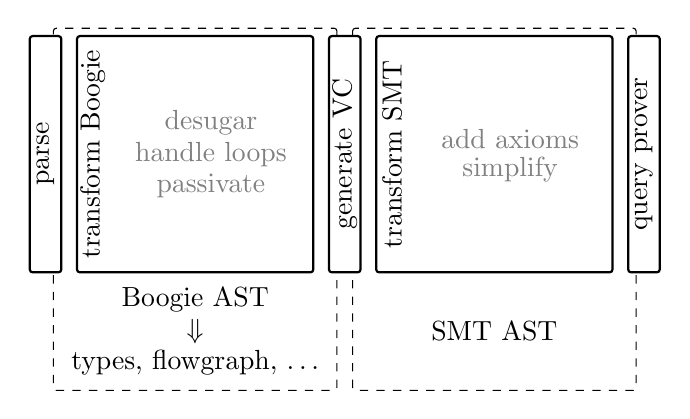
\begin{tikzpicture}
  \tikzstyle dr=[dashed,rounded corners=1pt,fill=white];
  \tikzstyle ar=[thick,rounded corners=1pt,fill=white];
  \tikzstyle g=[color=gray];
  \def\a{0.2}
  \def\b{1.5}
  \def\c{0.2}
  \def\d{1.5}
  \def\e{0.1}

  % ds rectangles
  \draw[dr] (-\e,\d+\e) rectangle (-\a-\c-\b-\b-\c-\a+\e,-\d-\d);
  \draw[dr] (+\e,\d+\e) rectangle (+\a+\c+\b+\b+\c+\a-\e,-\d-\d);

  % action rectangles
  \draw[ar] (-\a-\c-\b-\b-\c-\a-\a,-\d) rectangle +(+\a+\a,+\d+\d);
  \draw[ar] (+\a+\c+\b+\b+\c+\a+\a,+\d) rectangle +(-\a-\a,-\d-\d);
  \draw[ar] (-\a-\c-\b-\b,-\d) rectangle +(+\b+\b,+\d+\d);
  \draw[ar] (+\a+\c+\b+\b,+\d) rectangle +(-\b-\b,-\d-\d);
  \draw[ar] (-\a,-\d) rectangle +(\a+\a,\d+\d);

  % text
  \node[rotate=90] at (-\a-\c-\b-\b-\c-\a,0) {parse};
  \node[rotate=90] at (-\a-\c-\b-\b+\a,0) {transform Boogie};
  \node[rotate=90] at (0,0) {generate VC};
  \node[rotate=90] at (+\a+\c+\a,0) {transform SMT};
  \node[rotate=90] at (+\a+\c+\b+\b+\c+\a,0) {query prover};

  \node[g] at (-\a-\c-\b+\a,\a+\a) {desugar};
  \node[g] at (-\a-\c-\b+\a,0) {handle loops};
  \node[g] at (-\a-\c-\b+\a,-\a-\a) {passivate};

  \node[g] at (+\a+\c+\b+\a,\a) {add axioms};
  \node[g] at (+\a+\c+\b+\a,-\a) {simplify};

  \node at (-\a-\c-\b,-\d-\d/2+\a+\a) {Boogie AST};
  \node at (-\a-\c-\b,-\d-\d/2) {$\Downarrow$};
  \node at (-\a-\c-\b,-\d-\d/2-\a-\a) {types, flowgraph, $\ldots$};
  \node at (+\a+\c+\b,-\d-\d/2) {SMT AST};
\end{tikzpicture}
\caption{The architecture of FreeBoogie}\label{fig:architecture}
\end{figure} % >>>

The other important packages are: \method{parser}, which contains a parser
for Boogie; \method{ast}, which contains the Boogie AST data structures;
and \method{backend}, which contains everything involving SMT.

By design, Boogie transformers modify the AST as little as possible, are
sound, and, if possible, complete. (In other words, any unsoundness is a
bug, not a feature.) Because transformers do little, they are small, easy
to understand, probably correct. The most likely source of bugs is the
tacit dependencies between transformers. For example,
\method{vcgen.WeakestPrecondition} assumes that its input has no
assignments, and says so in its comments. Because of these dependencies,
the order in which transformers are applied, which is established in
\method{Main#initialize}, is important and fragile. A better solution is
needed.

% >>>
\section{Boogie AST and Transformers} % <<<
\label{sec:ast}

This section describes the package \method{ast}.

\subsection{The Boogie AST} % <<<

To understand Boogie's AST one must understand Boogie's abstract grammar,
which is in the file \texttt{fb.ag}, and the template for the AST data
structures, which is in the file \texttt{classes.tpl}.

AstGen, a helper tool hosted in the same repository, generates Java from
\texttt{fb.ag} and \texttt{classes.tpl}.  The approach has advantages and
disadvantages.  The generated classes are very similar to each other
because they come from the same template. This means that it is easy to
learn their interface.  It also means that it is easier to change all the
classes in a consistent way by changing the template.  The
$\approx360$~lines of \texttt{fb.ag} and \texttt{classes.tpl} are much
easier to understand than the $\approx6400$~lines of generated Java. Also,
it is relatively easy to modify the AST\null.  However, the programmer
needs to learn two small languages (for describing abstract grammars and
for writing templates), and IDEs are often confused by code generators.
Also, all operations on the AST \emph{must} be implemented using
visitors~\cite[Chapter~5]{gamma1995}, because one cannot add custom code
to particular AST classes.

To instantiate an AST class~$A$, programmers should say
\[x=A.\mathit{mk}(\langle\mathit{children}\rangle[,\langle\mathit{location}\rangle]).\]
To access a child~$c$ say $x.c()$. To create another instance of~$A$ that
is like~$x$, except that child~$c$ has value~$y$, say $x.withC(y)$.  It is
not possible to mutate an AST object (see Section~\ref{sec:immutability}).
Finally, one should get familiar with the operations defined in
\texttt{utils.tpl}, because they abstract idioms that occur frequently.

% >>>
\subsection{Visitors, Evaluators, Transformers} % <<<
\label{sec:visitors}

AstGen generates $\approx4000$~lines of Java code that makes it easier to
write Boogie transformers. For example, the $6$~lines in
Fig.~\ref{lst:example-transformer} are all that is needed to change all
occurrences of~$u$ into~$v$ in some Boogie AST\null. Note that the code is
fairly robust to changes in FreeBoogie's abstract grammar---as long as the
non-terminal is called \textit{Identifier}, it does not matter where
exactly it can appear in the program.

\bc
\begin{jml}
public class Renamer extends Transformer {
  @Override public Identifier eval(Identifier identifier) {
    if (!identifier.id().equals("u")) return identifier;
    else return Identifier.mk("v");
  }
}
\end{jml}
\ec{Changing all occurrences of variable~$v$ into variable~$y$}
{lst:example-transformer}

The root of the AST class hierarchy is \textit{Ast}; the root of the
visitors' class hierarchy is $\mathit{Evaluator}\langle R\rangle$, which is
generated from \texttt{evaluator.tpl}. For each class~$A$ that extends
\textit{Ast}, there is a method $R\,\mathit{eval}(A)$. For example, the
typechecker is an instance of
$\mathit{Evaluator}\langle\mathit{Type}\rangle$. Its \textit{eval}
methods return an instance of \textit{Type} when $A$~extends
\textit{Expr} (which itself extends \textit{Ast}), otherwise they return
\textbf{null}.

The \textit{eval} methods defined in \textit{Evaluator} recursively invoke
the current visitor on all the children and then return \textbf{null}.
This Fig.~\ref{lst:example-transformer} needs no code to traverse the
AST\null. \textit{Evaluator} also contains a cache that may be used by its
subclasses to avoid redoing work. See, for example,
\textit{AssociativeEvaluator} in \texttt{evaluator.tpl}, or the evaluation
of expressions in \method{tc.TypeChecker}.

Boogie transformers are a special case of evaluators: The class
\textit{Transformer} extends $\mathit{Evaluator}\langle\mathit{Ast}\rangle$
and is generated from \texttt{transformer.tpl}. The main functionality
implemented in \textit{Transformer}, path copying, is illustrated in
Figure~\ref{fig:path-copying}. Empty nodes (\tikz[baseline=-.5ex]
\node[fgdraw,circle] {}; and \tikz[baseline=-.5ex] \node[fgdraw]{};)
represent AST nodes that exist on the heap before a transformer~$T$ acts;
filled nodes (\tikz[baseline=-.5ex] \node[fgdraw,fgfill,circle]{}; and
\tikz[baseline=-.5ex] \node[fgdraw,fgfill]{};) represent AST nodes created
by the transformer~$T$. Because the transformer~$T$ is interested only in
rectangle nodes, it overrides only the \jmlCode|eval| method that takes
rectangles as parameters. That overriden method is responsible for creating
the filled rectangle (\tikz[baseline=-.5ex] \node[fgdraw,fgfill]{};). All
the other filled nodes (\tikz[baseline=-.5ex]
\node[fgdraw,fgfill,circle]{};) are created by \textit{Transformer}, and
need not be of any concern to the particular transformer~$T$.  The input
and the output of a transformer are treees that usually share a large
number of nodes.

\begin{figure}\centering % <<<
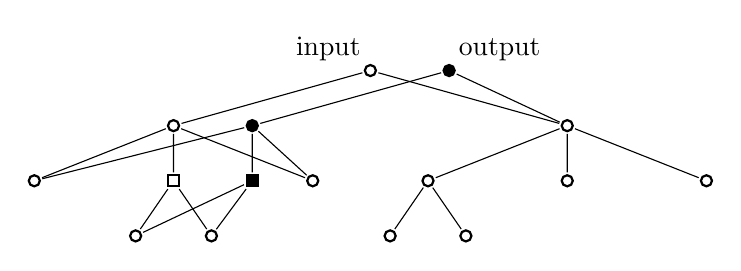
\begin{tikzpicture}
  [level distance=7mm,
  level/.style={sibling distance=5cm/(#1^1.5)}]
\tikzset{tree/.style={fgdraw,circle}}
\node[tree] (A) {}
  child {node[tree] (B) {}
    child {node[tree] (B1) {}}
    child {node[tree,rectangle] (C) {}
      child {node[tree] (C1) {}}
      child {node[tree] (C2) {}}
    }
    child {node[tree] (B3) {}}
  }
  child {node[tree] (A2) {}
    child {node[tree] {}
      child {node[tree] {}}
      child {node[tree] {}}
    }
    child {node[tree] {}}
    child {node[tree] {}}
  };
\path
  (A) +(1cm,0) node[tree,fgfill] (A') {}
  (B) +(1cm,0) node[tree,fgfill] (B') {}
  (C) +(1cm,0) node[tree,fgfill,rectangle] (C') {};
\draw (A') -- (B') -- (C');
\draw (A') -- (A2);
\draw (B') -- (B1); \draw (B') -- (B3);
\draw (C') -- (C1); \draw (C') -- (C2);
\node[above left] at (A) {input};
\node[above right] at (A') {output};
\end{tikzpicture}
\caption{Path copying}\label{fig:path-copying}
\end{figure} % >>>

Sometimes a transformer wants to `see' AST nodes of type~$A$
even if it computes no value for them. A typical example is
a pretty printer. In such cases a transformer may override
\jmlCode|eval(A)| and return \textbf{null}. A nicer solution is
to override \jmlCode|see(A)|, whose return type is \textbf{void}.
If both \jmlCode|eval(A)| and \jmlCode|see(A)| are overriden,
then the former will be called by the traversal code in
\textit{Transformer}.

% >>>
\subsection{Immutability} % <<<
\label{sec:immutability}

Many Java programmers dislike immutable data structures, so this design
decision needs some motivation.

A first objection is that immutable data structures lead to awkward code.
But I believe that the generated code, such as the \textit{withX} methods,
alleviate this problem.

A second objection is that immutable data structures are inefficient. The
equivalent of assigning a field is making a copy of a whole object. For
Boogie AST transformers, this means several objects must be copied
(Fig.~\ref{fig:path-copying}). However, note that one run of a transformer
over an AST tree with $n$~nodes takes $\Theta(n)$~time both for mutable and
for immutable data structures. The space usage of immutable ASTs is indeed
higher, unless the input of transformations needs to persist.

However, the advantages of immutability outweigh its
disadvantages.

First, immutability enables \textit{Evaluator} to cache the results of
previous computations, because only immutable data structures can be used
as keys in maps. Second, it turns out that there is a situation in which
the intermediate ASTs need to persist: For incremental verification.  And
third, immutability makes the code easier to understand, because it frees
the programmer from thinking about aliasing of AST nodes. In our
experience, aliasing of AST nodes inside a language-processing tool is a
wonderful source of bugs.

Still, there are situations when the programmer must think about aliasing
of Boogie AST objects. It is natural to think of an AST reference as
\emph{being} a piece of a Boogie program, even if, strictly speaking, it
only \emph{represents} a piece of a Boogie program. To maintain this useful
illusion the programmer must ensure that no sharing occurs \emph{within}
\emph{one} version of the AST\null. In practice, this means that the
programmer must occasionally clone pieces of the AST when implementing
transformers. To facilitate this, AstGen generates a \textit{clone} method
for each AST class.

Finally, let us note a technicality. Some AST nodes must contain lists of
other nodes. For example, a \textit{block} contains a list of
\textit{statement}s. There is no convenient way, however, to represent
immutable collections using Java's API. FreeBoogie uses the class
\textit{ImmutableList} from the Guava libraries~\cite{guava-libraries}
wherever \texttt{fb.ag} uses the \texttt{[list]} tag.

% >>>
% >>>
\section{Derived Information} % <<<

The package \textit{tc} derives extra information from a Boogie
AST---types, a symbol table, and a flowgraph.

The AST constructed by the parser is type-checked in order to catch simple
mistakes in the input. As a safeguard against bugs, the AST is type-checked
after each transformation. A side-effect of type-checking is that the type
of each expression is known.  The symbol table helps in navigating the
AST\null. It consists of one-to-many bidirectional maps that link
identifier declarations to places where the identifiers are used. These
maps are in \textit{SymbolTable} and in \textit{ImplementationChecker}.
Finally, it is sometimes convenient to view one implementation as a
flowgraph whose nodes are statements. Such a flowgraph is built by
\textit{FlowGraphMaker}.

All derived information is available through \textit{TcInterface}, the
facade of the package \textit{tc}.  Because of the caching in
\textit{Evaluator} and because much of the output of a transformation is
shared with the input, it is not expensive to re-derive the types and the
symbol table after each transformation.

% >>>
\section{Verification Condition Generation} % <<<

Boogie transformers reside in the package \textit{vcgen} (and use the
infrastructure in package \textit{ast}). Also, the key phase of FreeBoogie,
the generation of verification conditions, is implemented in the package
\textit{vcgen}.

The main quality of \textit{vcgen} is the simplicity of the code that does
the core task. If the reader reads no other code of FreeBoogie, we urge her
to take a look at the class \textit{StrongestPostcondition}.

To implement a new transformation, developers should a few more things.
First, there is a common pattern of keeping track of context. Second, there
are a few helper classes in this package as well.

Some transformations are local. For example, in order to turn
$\mathbf{havoc}\,x$ into $x:=\mathit{fresh}$ we need not know anything
about the surrounding code. Other transformations are only trivially
non-local. For example, in order to turn a \textbf{call} into
$\mathbf{assert}\ldots\mathbf{havoc}\ldots\mathbf{assume}$, one needs to
find the declaration of the procedure being called, which can be done using
the symbol table. However, transformers do sometimes need to keep track of
custom context information. For example, in order to desugar \textbf{break}
one needs to know the enclosing loops, and this ``derived information'' is
not available through \textit{TcInterface}. In those cases various
\textit{eval} methods will essentially send each other information through
fields of the transformer. The most complicated transformer, which
illustrates this technique, is \textit{AbstractPassivator}.

Transformers that need to replace a statement with a list of statements
extend \textit{CommandDesugarer}. Transformers that need to know which
variables are read or written in various pieces of program use the class
\textit{ReadWriteSetFinder}.

% >>>
\section{The Prover Backend} % <<<
\label{sec:backend}
% @review JRK *want*

The package \textit{backend} contains SMT data structures and code to
communicate with provers.

The SMT AST is a tree of strings---all the objects are of type
\textit{SmtTree}. However, to construct ASTs one \emph{should} use a
\textit{TermBuilder}, because its \textit{mk} methods perform
sort-checking. For example, to construct a conjunction between $x$~and~$y$
using the builder \textit{term}, one should write
$\mathit{term}.\mathit{mk}(\mathtt{"and"},x,y)$. For this to succeed, the
label \texttt{and} must have been declared before by calling \textit{def}
on the builder. That call has essentially the form \[
\mathit{term}.\mathit{def}(\langle\mathit{label}\rangle,
\langle\textit{sort of result}\rangle, \langle\textit{sorts of
arguments}\rangle). \] See \method{TermBuilder#TermBuilder} for examples.
All classes that implement the interface \textit{Prover} should know how to
handle all the labels that were registered with a term builder. See
\method{SimplifyProver#printTerm} for an example.

At the moment, \textit{TermOfExpr} and \textit{FormulaOfExpr} perform some
tricky maneuvers so that the output is understood by the old prover
Simplify, which does not understand \textbf{ite}. The trickiness will be
removed and Simplify no longer supported.

% >>>
\section{Related Work} % <<<

This paper evolved from Chapter~3 of the first author's PhD dissertation.

Leino~\cite{leino2008boogie} describes the Boogie language. Barnett et
al.~\cite{barnett2005boogie} describe the static verifier for Boogie
programs developed at Microsoft Research. It is part of the
Spec$^\sharp$~\cite{barnett2005spec} program verifier, and many other
static analysis tools. Barrett et al.~\cite{barrett2010lang} describes the
interface between verifiers and provers (reasoning engines), which
FreeBoogie adopts. B2BPL is a tool developed at ETH Z\"urich that converts
Java bytecode into Boogie. It is part of FreeBoogie's repository, because
we plan to integrate them.

% TODO: jSMTLIB

% >>>
\section{Conclusion} % <<<

FreeBoogie is an alternative to the Boogie tool. Its design stresses
correctness and simplicity. Even if at the moment it is only of $\alpha$
quality, we plan to keep improving it and we hope that it makes a good
framework for researchers that want to experiment with the Boogie language.

% >>>
\bibliographystyle{plain}
\bibliography{fb}
\end{document}
% vim:spell errorformat=%f\:%l-%m,%f\:%l\:%m,%f\:%m
% vim:tw=75:fo+=t:fmr=<<<,>>>:
